\documentclass[9pt,twocolumn,twoside,lineno]{pnas-new}
% Use the lineno option to display guide line numbers if required.

\usepackage[LGR,T1]{fontenc}
%\usepackage[latin9]{inputenc}
%\usepackage{geometry}
%\geometry{verbose,tmargin=1.75cm,bmargin=1.75cm,lmargin=2cm,rmargin=2cm}
\PassOptionsToPackage{natbib=true}{biblatex}
\usepackage{float}
\usepackage{amstext}
\usepackage{amssymb}
\usepackage{graphicx}
\usepackage{setspace}


%%%%%%%%%%%%%%%%%%%%%%%%%%%%%% to define \mu.
\DeclareRobustCommand{\greektext}{%
  \fontencoding{LGR}\selectfont\def\encodingdefault{LGR}}
\DeclareRobustCommand{\textgreek}[1]{\leavevmode{\greektext #1}}
\ProvideTextCommand{\~}{LGR}[1]{\char126#1}

\templatetype{pnasresearcharticle} % Choose template 

\title{Strong self-regulation and widespread facilitative interactions between
genera of phytoplankton}

% Use letters for affiliations, numbers to show equal authorship (if applicable) and to indicate the corresponding author
\author[a]{Coralie Picoche}
\author[a,b,1]{Frédéric Barraquand} 

\affil[a]{University of
Bordeaux, Integrative and Theoretical Ecology, LabEx COTE, Bât. B2
- Allée Geoffroy St-Hilaire, 33615 Pessac, France}
\affil[b]{CNRS, Institute
of Mathematics of Bordeaux, 351 Cours de la Libération, 33405 Talence,
France}

\leadauthor{Picoche \& Barraquand} %very small change l.224 on pnas-new.cls to avoid the 'et al.'

% Please add here a significance statement to explain the relevance of your work
\significancestatement{The continued coexistence of multiple species of phytoplankton in spite of likely competition is a long-standing puzzle of ecology, the so-called paradox of the plankton. Based on the long-time monitoring of 10 coastal study sites every two weeks over 20 years, we explore how biotic interactions shape the diversity of phytoplanktonic communities. We reveal that niche differentiation rather than neutral processes promotes coexistence. Moreover, although competition is often thought to dominate in phytoplanktonic systems, we show that a majority of interactions are in fact facilitative. We suggest that both strong niche differentiation and facilitation hold the key to the phytoplankton coexistence paradox.}

% Please include corresponding author, author contribution and author declaration information
\authorcontributions{C.P. and F.B. contributed equally to the project design. C.P. wrote the code for the analyses. F.B. and C.P. interpreted the results and wrote the manuscript.}
\authordeclaration{Authors declare no conflict of interest.}
%\equalauthors{\textsuperscript{1}C.P. and F.B. contributed equally to this work}
\correspondingauthor{\textsuperscript{1}To whom correspondence should be addressed. E-mail: frederic.barraquand@u-bordeaux.fr}
%\interfootnotelinepenalty=10000 %?????
% Keywords are not mandatory, but authors are strongly encouraged to provide them. If provided, please include two to five keywords, separated by the pipe symbol, e.g:
\keywords{phytoplankton $|$ coexistence $|$ time series $|$ niche theory $|$ networks} 

\begin{abstract}
The persistence of phytoplanktonic diversity in spite
of competition for basic resources has long been a source of wonder
and inspiration to ecologists. To sort out, among the many coexistence
mechanisms suggested by theory and experiments, which ones actually
maintain diversity in natural ecosystems, long-term field studies
are paramount. Here, we analyse a large dataset of phytoplankton abundance
time series, counted every two weeks over 20 years, at 10 sites along
the French coastline. We estimate biotic interactions using dynamic,
multispecies autoregressive models. We show that a strong self-regulation,
with competition strength within a genus an order of magnitude higher
than between genera, was present in all phytoplanktonic interaction
networks. Furthermore, the fraction of positive net effects between phytoplanktonic
taxa was above 50\% of non-zero interactions on average and at least 40\% in all sites.
Both strong self-regulation and widespread net facilitation should
therefore be key features of coexistence mechanisms intending to explain
phytoplankton diversity maintenance.
\end{abstract}

\dates{This manuscript was compiled on \today}
%\doi{\url{www.pnas.org/cgi/doi/10.1073/pnas.XXXXXXXXXX}}

\begin{document}

\maketitle
\thispagestyle{firststyle}
\ifthenelse{\boolean{shortarticle}}{\ifthenelse{\boolean{singlecolumn}}{\abscontentformatted}{\abscontent}}{}

% If your first paragraph (i.e. with the \dropcap) contains a list environment (quote, quotation, theorem, definition, enumerate, itemize...), the line after the list may have some extra indentation. If this is the case, add \parshape=0 to the end of the list environment.
\dropcap{H}ow species or close genera can coexist together in spite of competition
is one of the main puzzles of community ecology, especially for primary
producers that seemingly share the same basic resources \cite{hutchinson_paradox_1961}.
Many theoretical studies of competition models have shown that competitive
exclusion is likely in those circumstances \cite{armstrong1980competitive,chesson_updates_2018},
unless mechanisms involving spatial or temporal variation are at play \cite{armstrong1976coexistence,chesson_roles_1997,huisman_biological_2001,li_effects_2016}.
Neutral theory, that assumes a non-equilibrium coexistence maintained
by dispersal and equal competitive abilities for all species
(\citenum{hubbell_unified_2001}, though there are exceptions, see \citenum{volkov_neutral_2003,volkov_patterns_2007})
has been proposed as a solution to explain highly diverse communities \cite{hubbell_unified_2001,rosindell2011unified}.

However, the evidence gathered from terrestrial plant communities
starts to suggest that, in fact, niche rather than neutral processes
may be paramount to explain coexistence, with intraspecific competition
dwarfing interspecific competition in most cases \cite{adler_coexistence_2010,adler_competition_2018}.
Whether these conclusions drawn from studies of annual plants and
forest trees apply to other ecosystems and taxa is currently little
known (but see Mutshinda et al., \citenum{mutshinda_what_2009}).

Moreover, even within a single trophic level, competition may not
be the rule: the meta-analysis by Adler et al. \cite{adler_competition_2018}
reported a large number of facilitative interactions (30\%) and several
reviews \cite{brooker_facilitation_2008,mcintire2014facilitation}
have highlighted that facilitation may be much more widespread than
ecologists usually tend to think. Although some theoretical studies
suggest that facilitative interactions can be destabilizing (\emph{sensu}
resilience) and therefore undermine coexistence in Lotka-Volterra
models \cite{coyte_ecology_2015}, multiple other modelling \cite{gross_positive_2008}
and empirical \cite{brooker_facilitation_2008,cavieres2009facilitative}
studies have suggested that facilitative interactions can to a large
degree benefit coexistence, especially when multiple interaction types
are considered simultaneously \cite{mougi2012diversity,garcia2018effect}.

Here, we study a large multi-species dataset consisting of several
multivariate long-term time series of phytoplankton dynamics along
the French coastline, which we then analyse using multivariate autoregressive
(MAR) time series models, allowing for interactions between genera.
Although many ecological studies focus on interactions between species,
competition has been shown experimentally to occur between different
genera of phytoplankton \cite{titman_ecological_1976,descamps-julien_stable_2005}.
The genus level is also a rather fine taxonomic scale for phytoplankton
interaction studies, as most studies are restricted to interaction
between different classes or even phyla \cite{ives_estimating_2003,hampton_sixty_2008,griffiths_phytoplankton_2015}.
Studying interactions between different genera of phytoplankton therefore
both makes empirical sense in light of competition experiments and
allows to estimate better-resolved networks. We focus here on genera
that belong mostly to diatoms and dinoflagellates. To put our results
into a more general context, we then compare our interaction strength
estimates to previously published interaction networks produced under
the same statistical framework, both in plankton and other empirical
systems. 

%Note: please start your introduction without including the word ``Introduction'' as a section heading (except for math articles in the Physical Sciences section); this heading is implied in the first paragraphs. 

\section*{Results}
\subsection*{Interaction estimates}

\begin{figure*}[ht!]
\centering
 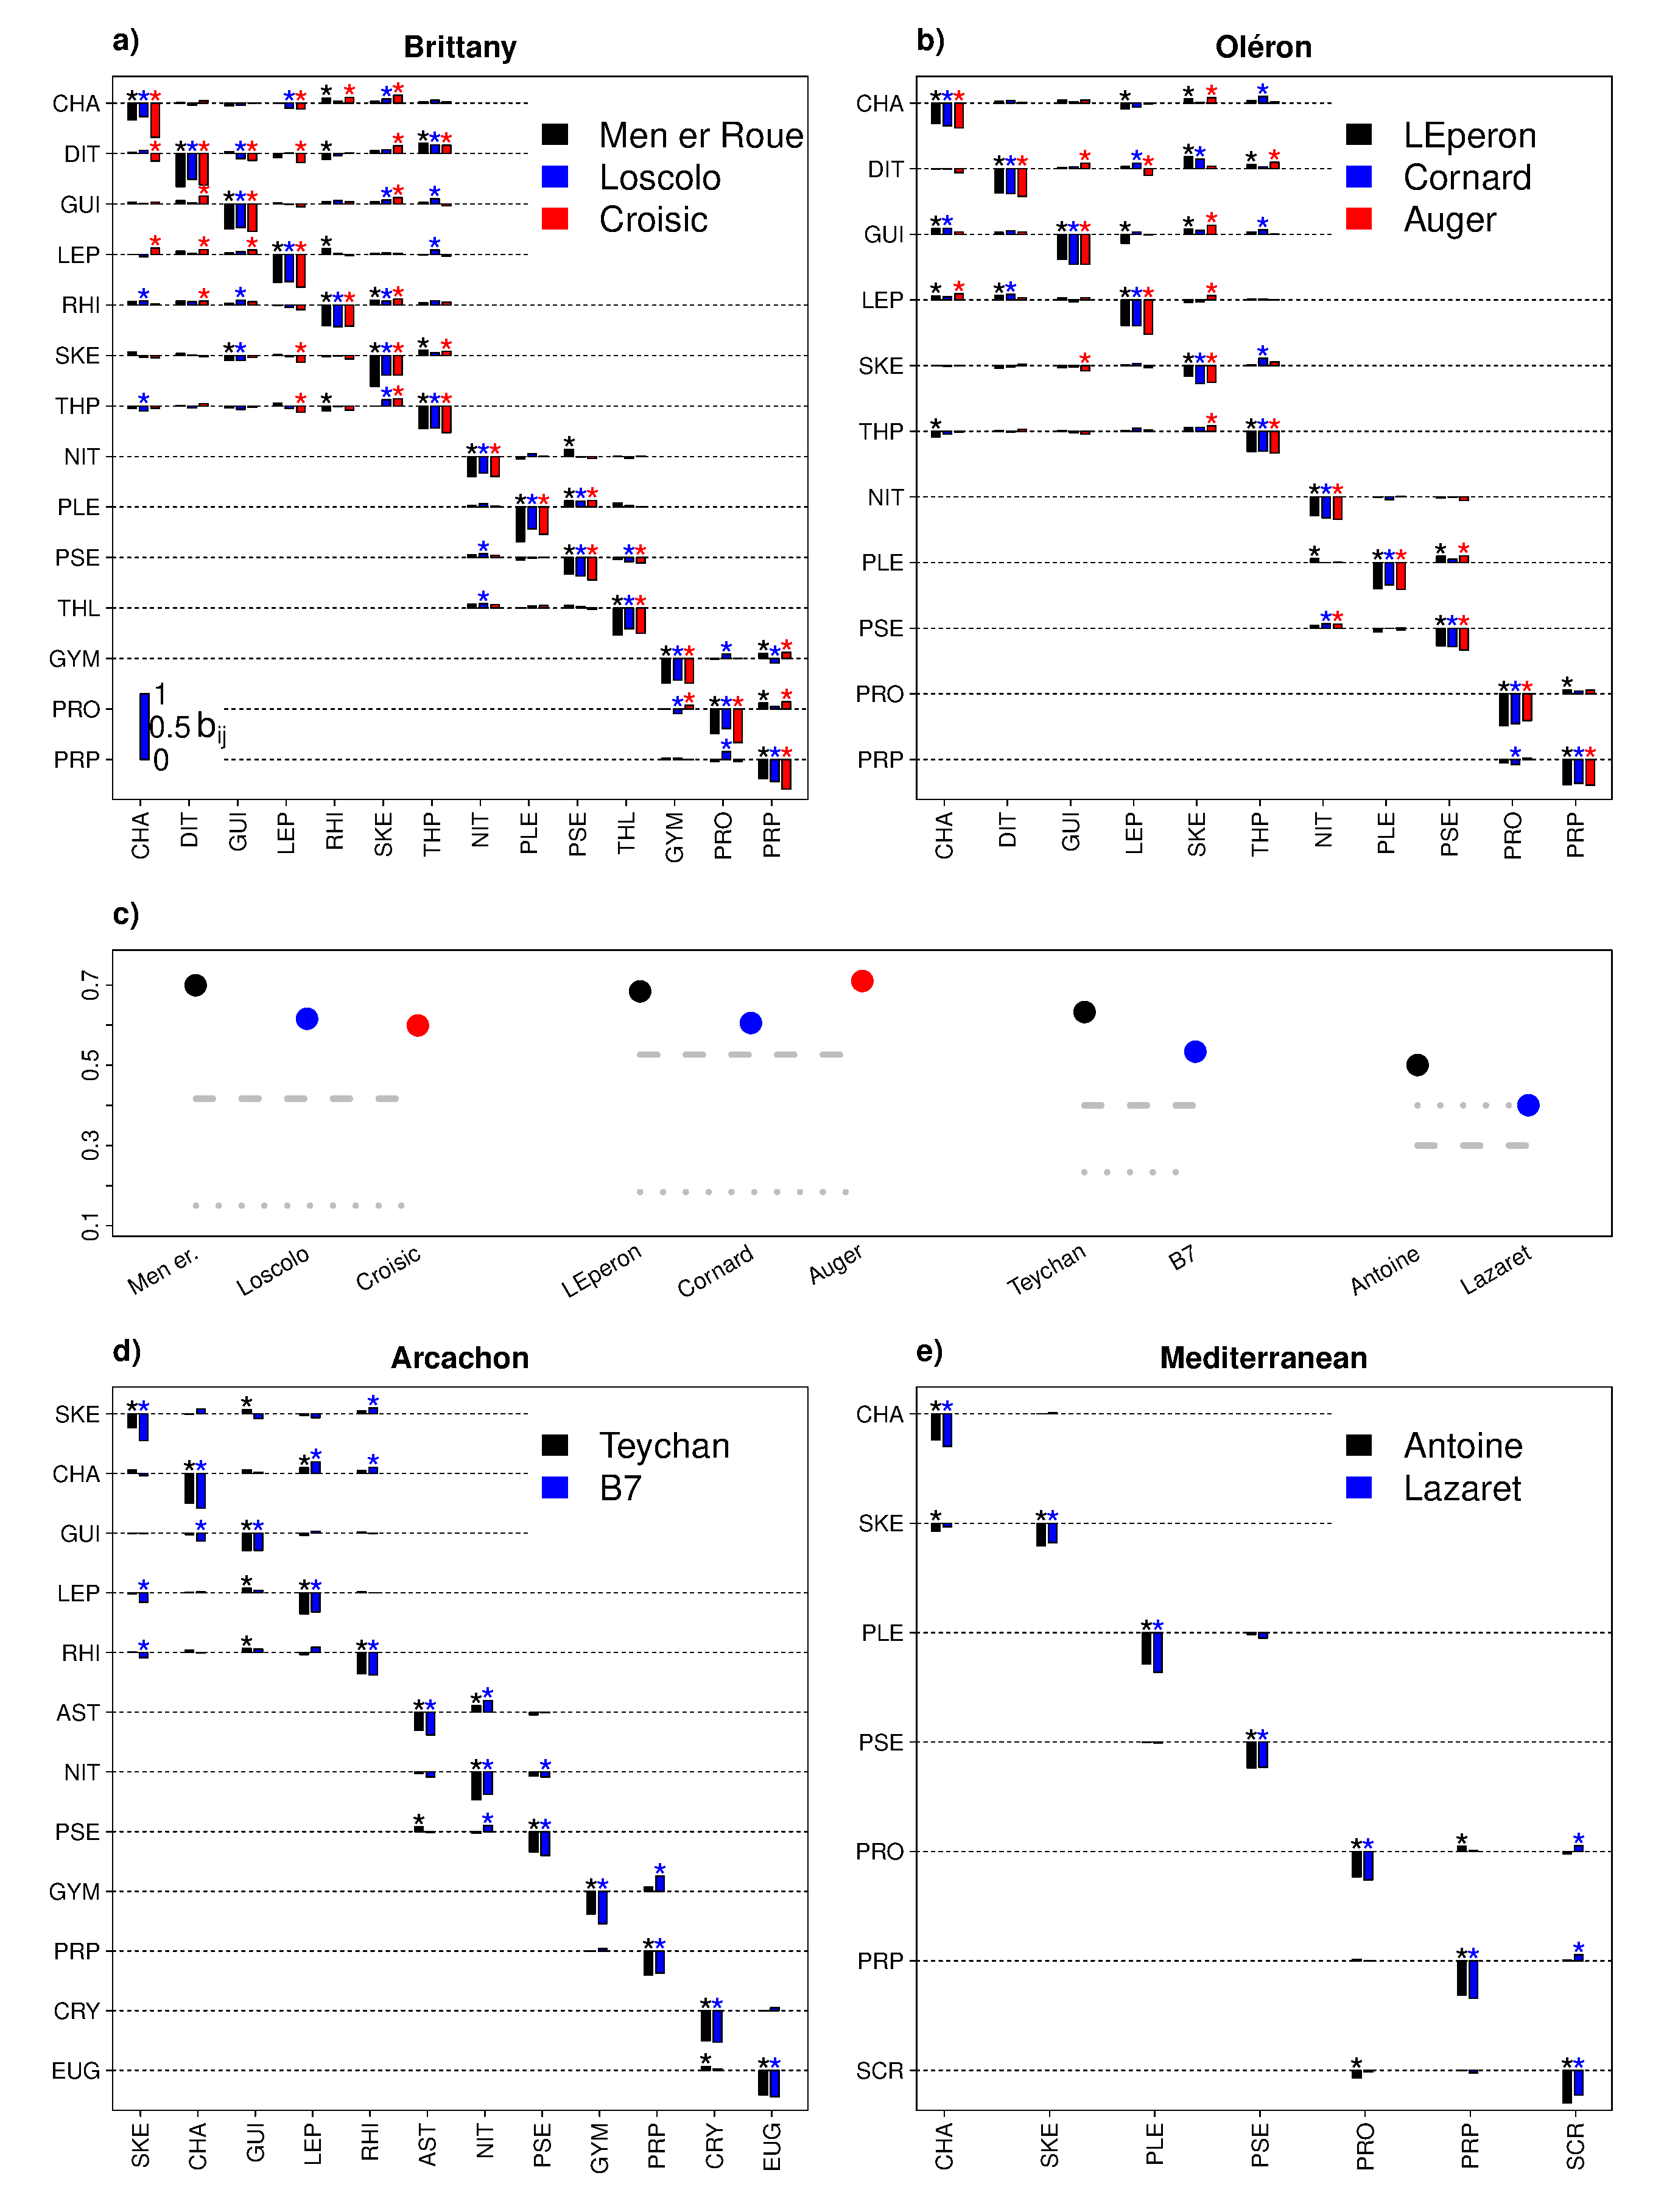
\includegraphics[width=15.8cm]{biotic_interaction_matrices_MainFig_allin1_v4}
\caption{Interaction matrices estimated in 10 sites along the French
coastline. Four regions are distinguished: Brittany (a), Oléron (b),
Arcachon (d) and the Mediterranean Sea (e). Only interactions between
clades (pennate and centric diatoms, dinoflagellates, other planktonic
taxa) are allowed, as this is the best fitting interaction scenario
(SI Appendix, Fig.~S3). Taxon $j$ (in columns) has an effect illustrated
by the bar height on taxon $i$'s growth rate (in rows). We present
the interaction matrix minus the identity matrix ($\mathbf{B}-\mathbf{I}$)
because this compares unambigously intra- and intergenera interactions.
The scale for the coefficient values is given at the bottom left of
panel a). 95\% significance of coefficients is marked by asterisks
({*}). The community composition is given in SI Appendix, Table~S2.
The fraction of positive interactions in each matrix is given by points
in c) while the dashed (resp., dotted) line represents the ratio of
interactions remaining positive (resp., negative) for all sites of
a given region.}
\label{fig:Interaction-matrices}
\end{figure*}

\begin{figure*}[!h]
\centering
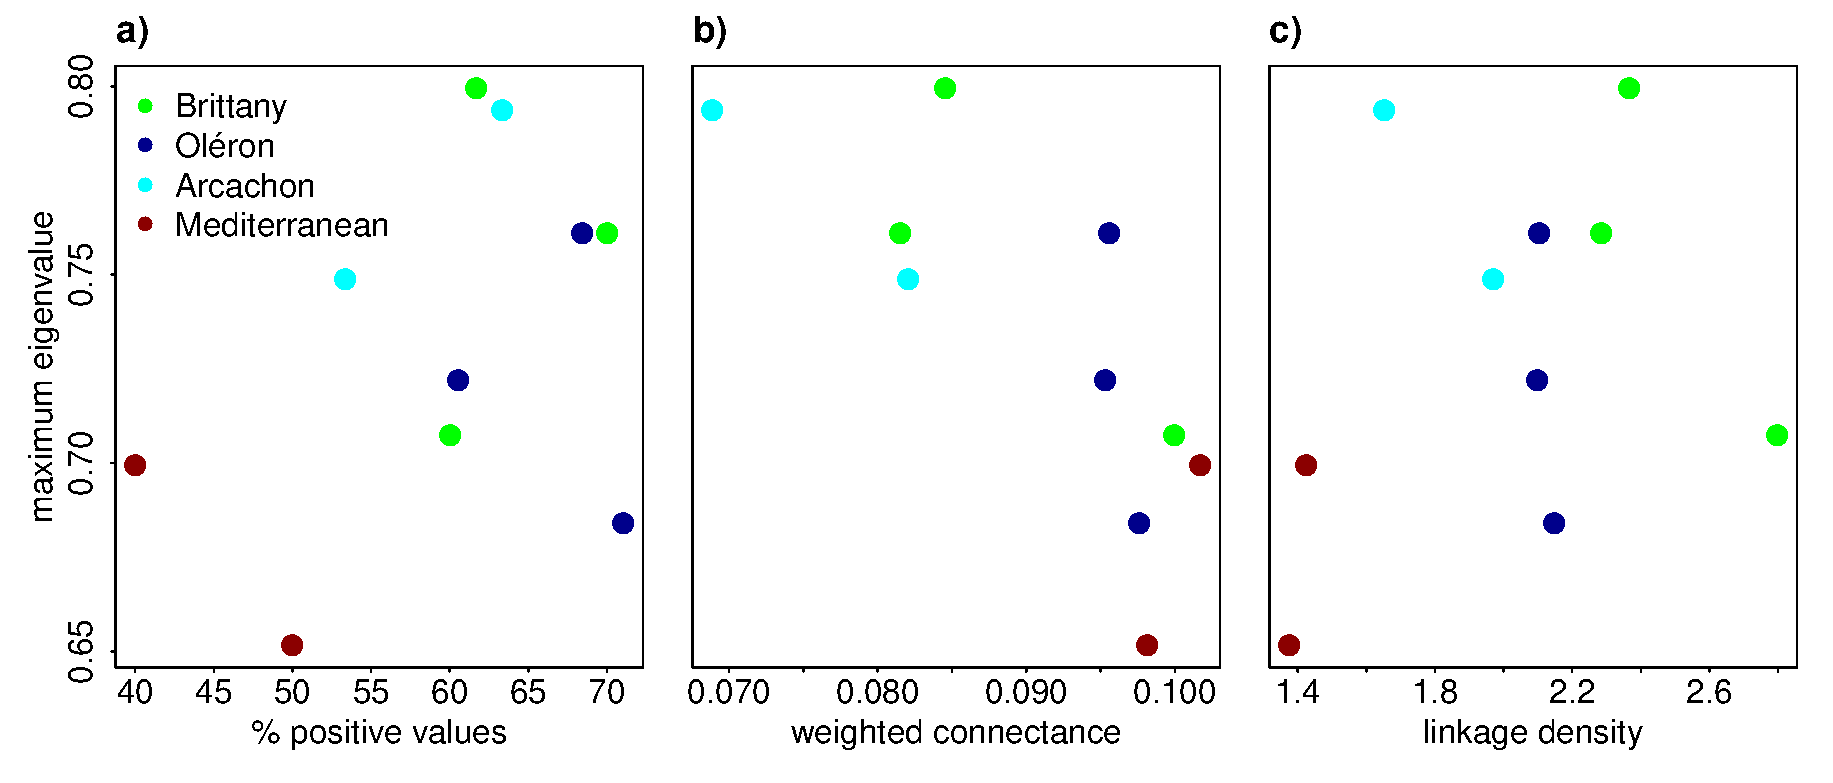
\includegraphics[width=17.8cm]{complexity_stability_MainFig_pencenjustB}
\caption{Relation between stability and complexity of the interaction
networks. The maximum modulus of the interaction matrix $\mathbf{B}$
eigenvalues indicates stability \emph{sensu} resilience. Each point
color corresponds to a given region. Metrics formula for weighted
connectance and linkage density are given in SI Appendix.}
\label{fig:Stability-community}
\end{figure*}

Using MAR(1) autoregressive models, we have produced interaction matrices \cite{ives_estimating_2003,hampton2013quantifying}
-- i.e., Jacobian community matrices on the logarithmic scale \cite{ives_estimating_2003}.
Best-fitting models corresponded to a phylogenetically-structured
interaction scenario, where interaction only occurred betwen closely
related genera (SI Appendix, Fig.~S3). This led to sparse, modular
matrices that have two main features. First, we observe a strong self-regulation
for all sites (Fig.~\ref{fig:Interaction-matrices}, diagonal elements
of all matrices), a feature that we have previously highlighted in
a more detailed analysis on one of the considered study regions \cite{barraquand_coastal_2018}.
The ratio of mean intragenus to intergenus interaction coefficients
varies between 6 and 10, not counting coefficients set to 0 in the
estimation process. If we include the zeroes in the interaction matrix
in the computation of the intra/inter mean interaction strength, the
ratio rises to 21-43. Therefore, intragenus interactions are on average
much stronger than intergenus interactions, approximately 10 to 20
times stronger.

Second, although the percentage of facilitative interactions seemed
to vary among sites (between 40\% and 71\% of interactions in the
selected models), facilitation remained predominant in 9 sites out
of 10 (only Lazaret, in the Mediterranean Sea, has 60\% negative interactions).
Our observational setup being nested, with sites within regions, we
can examine whether locally positive interactions remain positive
in a regional context: the percentage of consistently positive interactions
at the regional level varies between 30\% and 53\%, higher than the
percentage of similarly defined negative interactions (between 15\%
and 40\%), except for sites in the Mediterranean Sea.

We have found that the percentage of true mutualism (+/+) is substantial:
averaged over all sites, 32\% of all interactions are (+/+) while
only 12\% of them are (-/-), see also SI Appendix, Fig. S5. The sign
correspondence is not always maintained between French regions: the
only interaction that is non-zero in the 10 sites (CHA/SKE) is mutualistic
in Men er Roue only (Brittany) and mixed (+/-) at all other sites.
Within the same region, however, interactions measured at different
sites tend to keep the same sign. In the 3 sites of Oléron, for instance,
there were 4 interactions which remained positive on both sides (CHA/GUI,
DIT/GUI, LEP/THP, SKE/THP), 3 of them being also mutualistic in some
of the Brittany sites. This contradicts previous observations that
mutualistic interactions tend to be more context-dependent than competitive
interactions \cite{chamberlain_how_2014}. 


\subsection*{Interaction network analysis}

The stability (\emph{sensu} resilience, \citenum{ives_stability_2007})
of all interaction matrices was not strongly affected by the percentage
of positive interactions or their connectivity properties (Fig.~\ref{fig:Stability-community}).
The maximum modulus of the interaction matrix eigenvalues remained
between 0.65 and 0.80. There was also a slight increase in stability
with weighted connectance, with a drop in eigenvalue modulus for weighted
connectances between 0.09 and 0.1.

Given that a direct complexity-stability link was not obvious, we
investigated whether the matrix coefficients had some particular structure
that could help theoretical ecology to make better null models of
joint community dynamics and interactions \cite{james_constructing_2015}.
We defined two scores, vulnerability (summed effect of others on
the focal species growth rate, SI Appendix, Eq.~S5) and impact (summed
effect of the focal species onto other species growth rates, SI Appendix,
Eq.~S6). Relations between inter- and intra-genus interactions emerged
(Fig.~\ref{fig:Vulnerability_impact}): genera that were more self-regulating
also had also a higher vulnerability score and a lower impact score.
Those two influences are likely to trade-off: a high degree of self-regulation
somehow buffers outside influences. Taxa that were less self-regulating
were also more likely to have a broad range of effects onto other
taxa. As these genera tended to be more abundant (SI Appendix, Fig.~S7),
they were more likely to affect other genera. It is important to note,
however, that these trends are weak and there is therefore a considerable
amount of randomness dominating the interaction matrix: many scenarios
of self-regulation vs limitation by others are therefore possible.

\begin{figure*}[!h]
\centering
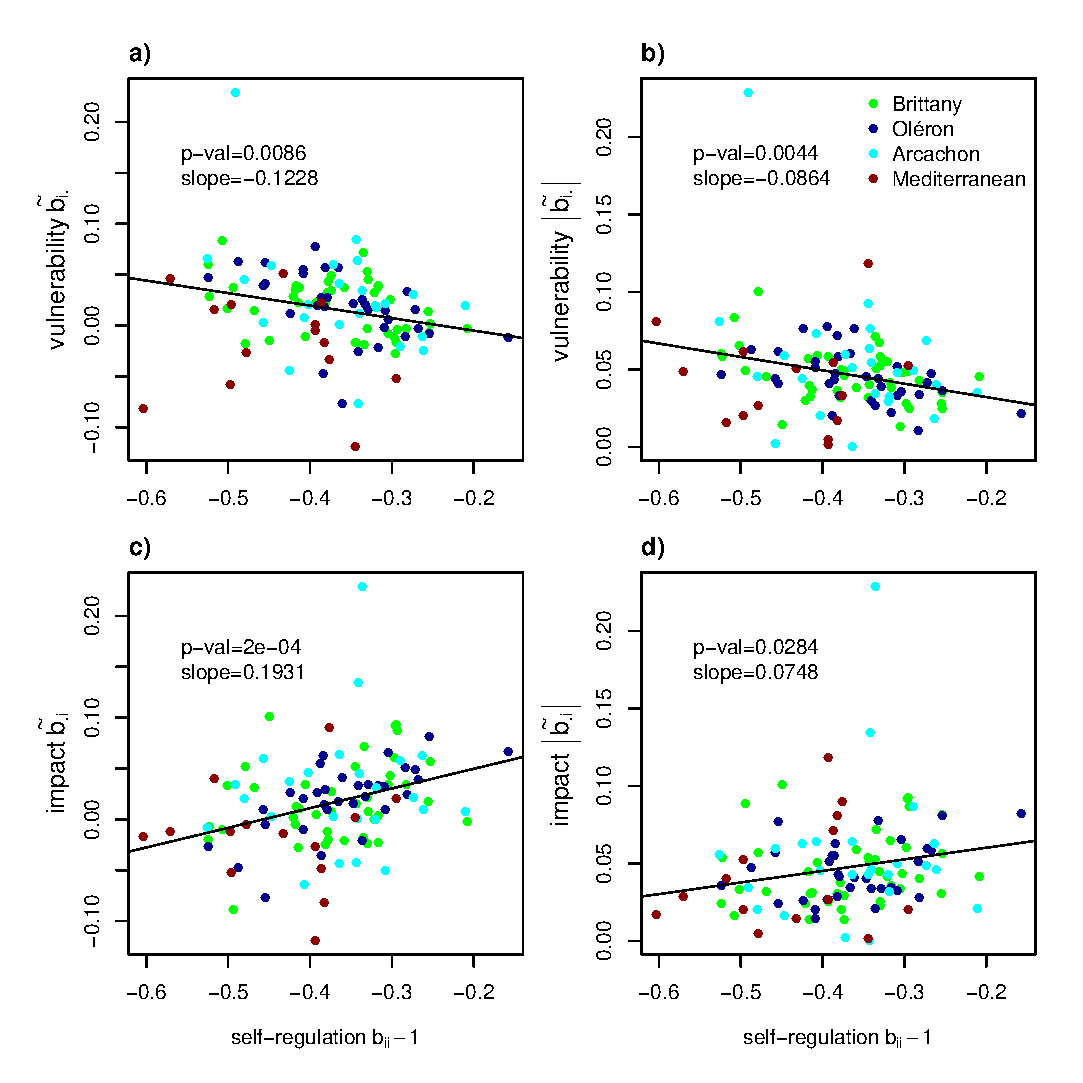
\includegraphics[width=17.8cm]{pencen_generality_vs_vulnerability_MainFig}
\caption{Relation between vulnerability/impact and self-regulation.
Average vulnerability (effects of others on the focal taxon growth
rate, a-b) and impact (effects of the focal taxon on others' growth
rates, c-d), as well as self-regulation, are computed for untransformed
(a-c) or absolute (b-d) values of the coefficients of the interaction
matrix ($\mathbf{B}-\mathbf{I}$) for the 10 study sites. Each color
corresponds to a given region (SI Appendix, Fig.~S1). The p-value
of the Pearson correlation between vulnerability (respectively impact)
and self-regulation is given in the top left of each panel and the
slope of the linear regression is given by the black line across scatter
plots.}
\label{fig:Vulnerability_impact}
\end{figure*}

Aside from these trade-offs, some of which promote some stability
(\emph{sensu} invariability, \citenum{Arnoldi431296}), we found no
remarkable patterns of covariation between matrix elements (other
than a mean-variance scaling of interaction coefficients, SI Appendix
Fig.~S6).

\subsection*{Literature comparison}

Finally, we sought to put these results in a broader context by compiling
the intra vs inter group estimates of previous MAR(1) studies of long-term
observational count data (listed in SI Appendix Table~S3). We found
that the order of magnitude of intra/inter interaction strengths considered
here is not particularly above those found for most planktonic systems
to which MAR(1) models have been fitted, considering that our systems
are relatively high-dimensional and that the higher the number of
taxa, the larger the intraspecific regulation \cite{barabas_self-regulation_2017}.
We included in Fig.~\ref{fig:meta_ratio} not only plankton studies
but also a couple of vertebrate or insect studies on less diverse
communities, where interactions are stronger. The conclusion from
this comparison seems to be that, unlike small communities that can
be tight-knit, any diverse system of competitors and facilitators
has evolved large niche differences making intragroup competition
much larger in magnitude than intergroup interactions.

\begin{figure*}[!h]
\centering
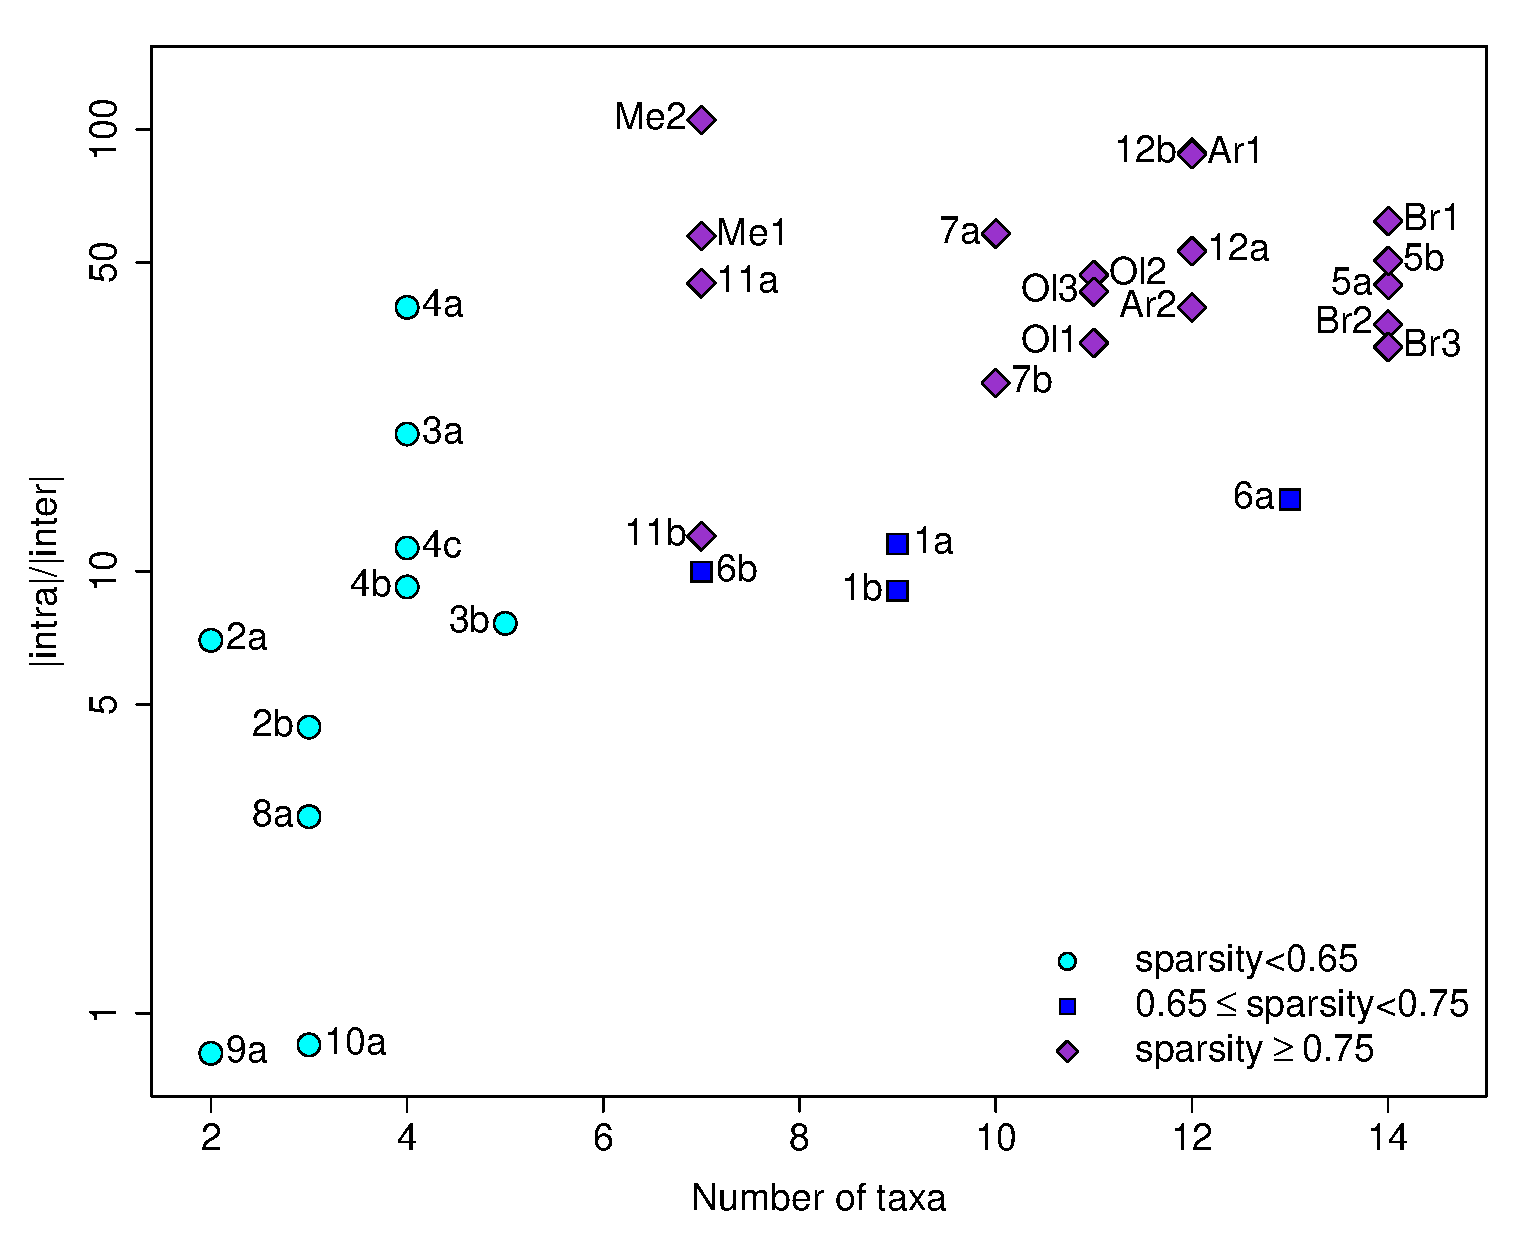
\includegraphics[width=0.8\linewidth]{Ratio_function_dim}
\caption{Ratio of intra- to inter-group interaction strength in Multivariate
AutoRegressive (MAR) models in the ecological literature as a function
of the number of species they include.The name of each studies,
corresponding to each code, is given in SI Appendix, Table~S3. Codes
beginning with letters correspond to the present study. The symbol
color and shape correspond to the sparsity of the interaction matrix
(e.g., the proportion of null interactions in the matrix). Intergroup
interactions were set to 0 when they were not specified in the articles
(in most cases, articles removed non-significant interactions at the
95\% threshold).} 
\label{fig:meta_ratio}
\end{figure*}

\section*{Discussion}

\subsection*{Strong self-regulation and facilitation}

We found very large niche differences between genera, translating
into much higher intragenus than intergenus effects on growth rates
(i.e., strong self-regulation), together with a high degree of facilitative
net interactions.

The rather high intra/intertaxon interaction strength ratio \cite{levine_importance_2009}
that we found, from 5 to 20, depending on how one counts the interactions
set to zero in the estimation process, could appear extremely high
in light of previous intra/interspecific competition strength estimates
of 4 to 5 by Adler et al. \cite{adler_competition_2018}. Even
though their model is a different one, i.e., Lotka-Volterra competition,
we prove in the SI Appendix that the intra/inter ratio
should remain commensurate. The difference in the intra/inter ratio
that we found should therefore lie elsewhere, which requires some
explanation. First, one could argue that such high intra/inter ratio
arises because we consider the genus as our baseline taxonomic unit,
rather than the species. Although it is logical that niche differentiation
increases as one gets up the phylogenetic tree, and that getting down
to the species level could slightly decrease that ratio, there are
two arguments suggesting that the niche differences found here extend
to the species level. First, species belonging to the various genera
considered here are often found to compete in experiments \cite{titman_ecological_1976,tilman_phytoplankton_1982,descamps-julien_stable_2005}.
There is therefore a massive difference between niches in the lab
and in the field \cite{barraquand_coastal_2018}. Second, the
only other study that managed to provide MAR(1) estimates down to
the species level for phytoplankton, that of Huber and Gaedke \cite{huber_role_2006},
provides an intra/interspecific strength ratio similar to ours (point
7a in Fig.~\ref{fig:meta_ratio}). Strong self-regulation seems therefore
a genuine feature of field phytoplanktonic communities.

Another main finding of our study is the large frequency of positive
interactions, with 30\% truly mutualistic (+/+) interactions and between
40 and 70\% facilitative effects. This again can be compared to the
meta-analysis by Adler et al.\cite{adler_competition_2018} who
also found facilitative interactions, but a little less than here
($\approx$30\%). However, Adler et al.\cite{adler_competition_2018}'s
review contains many experiments while the plant literature is replete
with field examples of facilitation \cite{brooker_facilitation_2008,mcintire2014facilitation},
so that plant facilitation could be higher in the field. At the moment,
it is therefore unknown how the predominance of facilitative interactions
that we found in phytoplankton compares to facilitation in terrestrial
plants. We note that several authors using MAR(1) models previously
forbade positive interactions within the same trophic level, so that
the fraction of facilitative interactions in plankton cannot be computed
from literature-derived MAR(1) estimates.

The large niche differences and facilitative interactions that arise
when considering a single trophic level are an emergent property,
arising from hidden effects of resources or predator partitioning/sharing \cite{chesson_updates_2018}.
In our previous publication investigating in detail the Arcachon study
sites \cite{barraquand_coastal_2018}, we have argued that for
phytoplankton, the strong intragroup density-dependence could arise
from effects of natural enemies \cite{haydon_pivotal_1994,barraquand_coastal_2018}.
Natural enemies could also very well create apparent mutualism between
prey species \cite{abrams_apparent_1998,barraquand_indirect_2015,de_ruiter_emergent_2017}.
We believe this to be likely true for the present study as well, given
that the new study regions (Oléron, Brittany, Mediterranean) have
similar predators to the Arcachon site (zooplankton \citenum{jamet_zooplankton_2001,moderan_zooplankton_2010,tortajada_network_2012})
and parasites (viruses \citenum{ory_pelagic_2010}, fungi). Though
natural enemies are good candidates to explain the observed niche
differences and emerging facilitation, one must bear in mind that
other known drivers of phytoplankton dynamics such as allelopathy \cite{felpeto_allelopathy_2018},
auxotrophy \cite{tang_most_2010} or hydrodynamics \cite{levy_role_2018}
can all, in theory, help create different niches and an emerging facilitation
(see last subsection of the Discussion). Finally, resources that are
usually considered limiting for all species might in fact not always
be: the changes in phytoplankton absorption spectrum documented by
Burson et al. \cite{burson_competition_2018} constitute an example
of fine-scale resource partitioning of one resource, light, that is
usually believed to be limiting for all species and genera.

\subsection*{No complexity-stability relationship but connections between self-regulation
and intergroup interactions}

There was no relation between the complexity of the communities (measured
as either the weighted connectance or linkage density of the interaction
matrices) and their stability, as measured by the dominant eigenvalue
of the interaction matrix, which measures the return time to a point
equilibrium. This result is conditional upon our model being a good
approximate description of the system (i.e., no multiyear limit cycles
or chaotic attractors as the mapping between eigenvalues and actual
stability is distorted in that case, \citenum{certain_how_2018}),
but we showed on a subset of this data that a fixed point in a MAR(1)
model, perturbed by seasonality and abiotic variables, is an accurate
description of the system \cite{barraquand_coastal_2018}. Therefore,
we are confident that the absence of complexity-resilience found here
is genuine. This absence of direct link between complexity and stability
could be an actual feature of empirical systems, as shown previously
by Jacquet et al. \cite{jacquet_no_2016} using a different technique,
even though it does contradict previous results on random matrices,
especially for competitive and/or mutualistic networks \cite{allesina_stability_2012}.
We also found that the percentage of mutualistic interactions, that
is thought to affect the stability of the network \cite{mougi2012diversity,coyte_ecology_2015,garcia-callejas_multiple_2018},
does not have a major impact on the network's resilience.

In addition to weighted connectance, indices at the network-level
(e.g., linkage density) and at the species or genus level (vulnerability
and impact) approximate the average effects exerted and sustained
by any given taxa in the different study sites. While, at the network
level, network structure (either complexity measures or the percentage
of mutualistic interactions) did not affect stability, a relation
emerged between self-regulation, necessary for coexistence, and genus-level
indices. We found that the more a genus is self-regulated, the more
it tends to be vulnerable to other genera impacts and the less it
impacts other genera. High self-regulation usually indicates large
niche differences with the rest of the community, and it makes therefore
sense that a species/genus whose needs strongly differ from the others
only marginally impacts the resources of the other coexisting species.
Furthermore, a low self-regulation was correlated with high average
abundance, which echoes findings by Yenni et al. \cite{yenni_persistent_2017}
who found that rare species usually show stronger self-regulation.
This correlation between rarity and self-regulation could explain
the lesser impact effect of high self-regulated species/genus: a species
which dominates the community composition can have a major effect
on the others, especially as they usually cover more space, while
it is harder for rare, localised species to have large impacts. However,
it was more difficult to explain the relationship between self-regulation
and vulnerability: a genus that is more self-regulated and rarer was
found here to be on average more vulnerable to other genera's increases
in densities. Such relation implies greater stability (\emph{sensu}
resilience) for the network as a whole, because the taxa that are
the most vulnerable to other taxa's impacts are also those whose dynamics
are intrinsically more buffered. By which mechanisms this could happen
is so far unclear and open to speculation. We caution, however, that
the relationships between vulnerability, impact and self-regulation
that we evidenced are all relatively weak: considerable stochasticity
dominates the distribution of interaction matrix coefficients.

\subsection*{Ghosts of competition past and present}

Overall, the dominance of niche differentiation in observational plankton
studies -- based on our analysis of the REPHY dataset and re-analysis
of the MAR(1) literature -- is similar to what has been recently
found in plant community studies \cite{volkov_patterns_2007,adler_competition_2018}
or empirical food webs including horizontal diversity \cite{barabas_self-regulation_2017}.
Large niche differences might be due to the ghost of the competition
past, i.e., competition has occurred in the past, leading to strong
selection and subsequent evolution leading to progressive niche separation.
In this scenario, species have evolved niches that allow them not
to compete or to interact only weakly (very strong facilitative effects
might be likewise destabilizing, \citenum{coyte_ecology_2015}). The
likely predator effects that we highlighted above could be comprised
within such niche differentiation \emph{sensu largo}: specialized
predators can make strong conspecific density-dependence emerge \cite{bagchi_pathogens_2014,comita_testing_2014},
while switching generalists can also promote diversity \cite{vallina2014maximal}.
Both predators and resources have often symmetrical effects and can
therefore contribute almost equally to such past niche differentiation \cite{chesson_updates_2018}.

An intriguing new possibility, dubbed the ``ghost of competition
present'' \cite{tuck_strong_2018}, suggests by contrast that
spatial distributions in relation to abiotic factors might have a
large impact on the interaction strengths inferred from temporal interaction
models such as ours. Recent combinations of model fitting and removal
experiments have shown that the model fitting usually underestimates
the effect of competitors that are uncovered by removal experiments \cite{tuck_strong_2018,adler_weak_2018}.
This could occur for instance if species are spatially segregated
(at a small scale) because each species only exists within a domain
where it is relatively competitive (Pacala's spatial segregation hypothesis \cite{pacala1997biologically}),
while a focal species could spread out if competitors were removed.
This means that a species can be limited by competitors, but act so
as to minimize competition (a little like avoidance behaviour in animals),
which implies that competition is in effect hard to detect when all
species are present. This would require spatial segregation between
phytoplankton species at the scale of interactions, i.e., at the microscale.
At the moment, it is known that turbulence generates inhomogeneities
at the microscale \cite{barton_impact_2014,breier_emergence_2018}
but it is quite unclear how this affects multivariate spatial patterns
of species distributions (\textit{sensu} Bolker and Pacala, \citenum{bolker_spatial_1999},
or Murrell and Law, \citenum{murrell_heteromyopia_2003}). Moreover,
even if turbulence generates spatial structure with segregation between
species, it is not quite clear that the ``ghost of competition present''
mechanism could work for plankton, because turbulence rather than
organism movement dictates where the phytoplankton patches can or
cannot appear.


% \begin{SCfigure*}[\sidecaptionrelwidth][!h]
% \centering
%  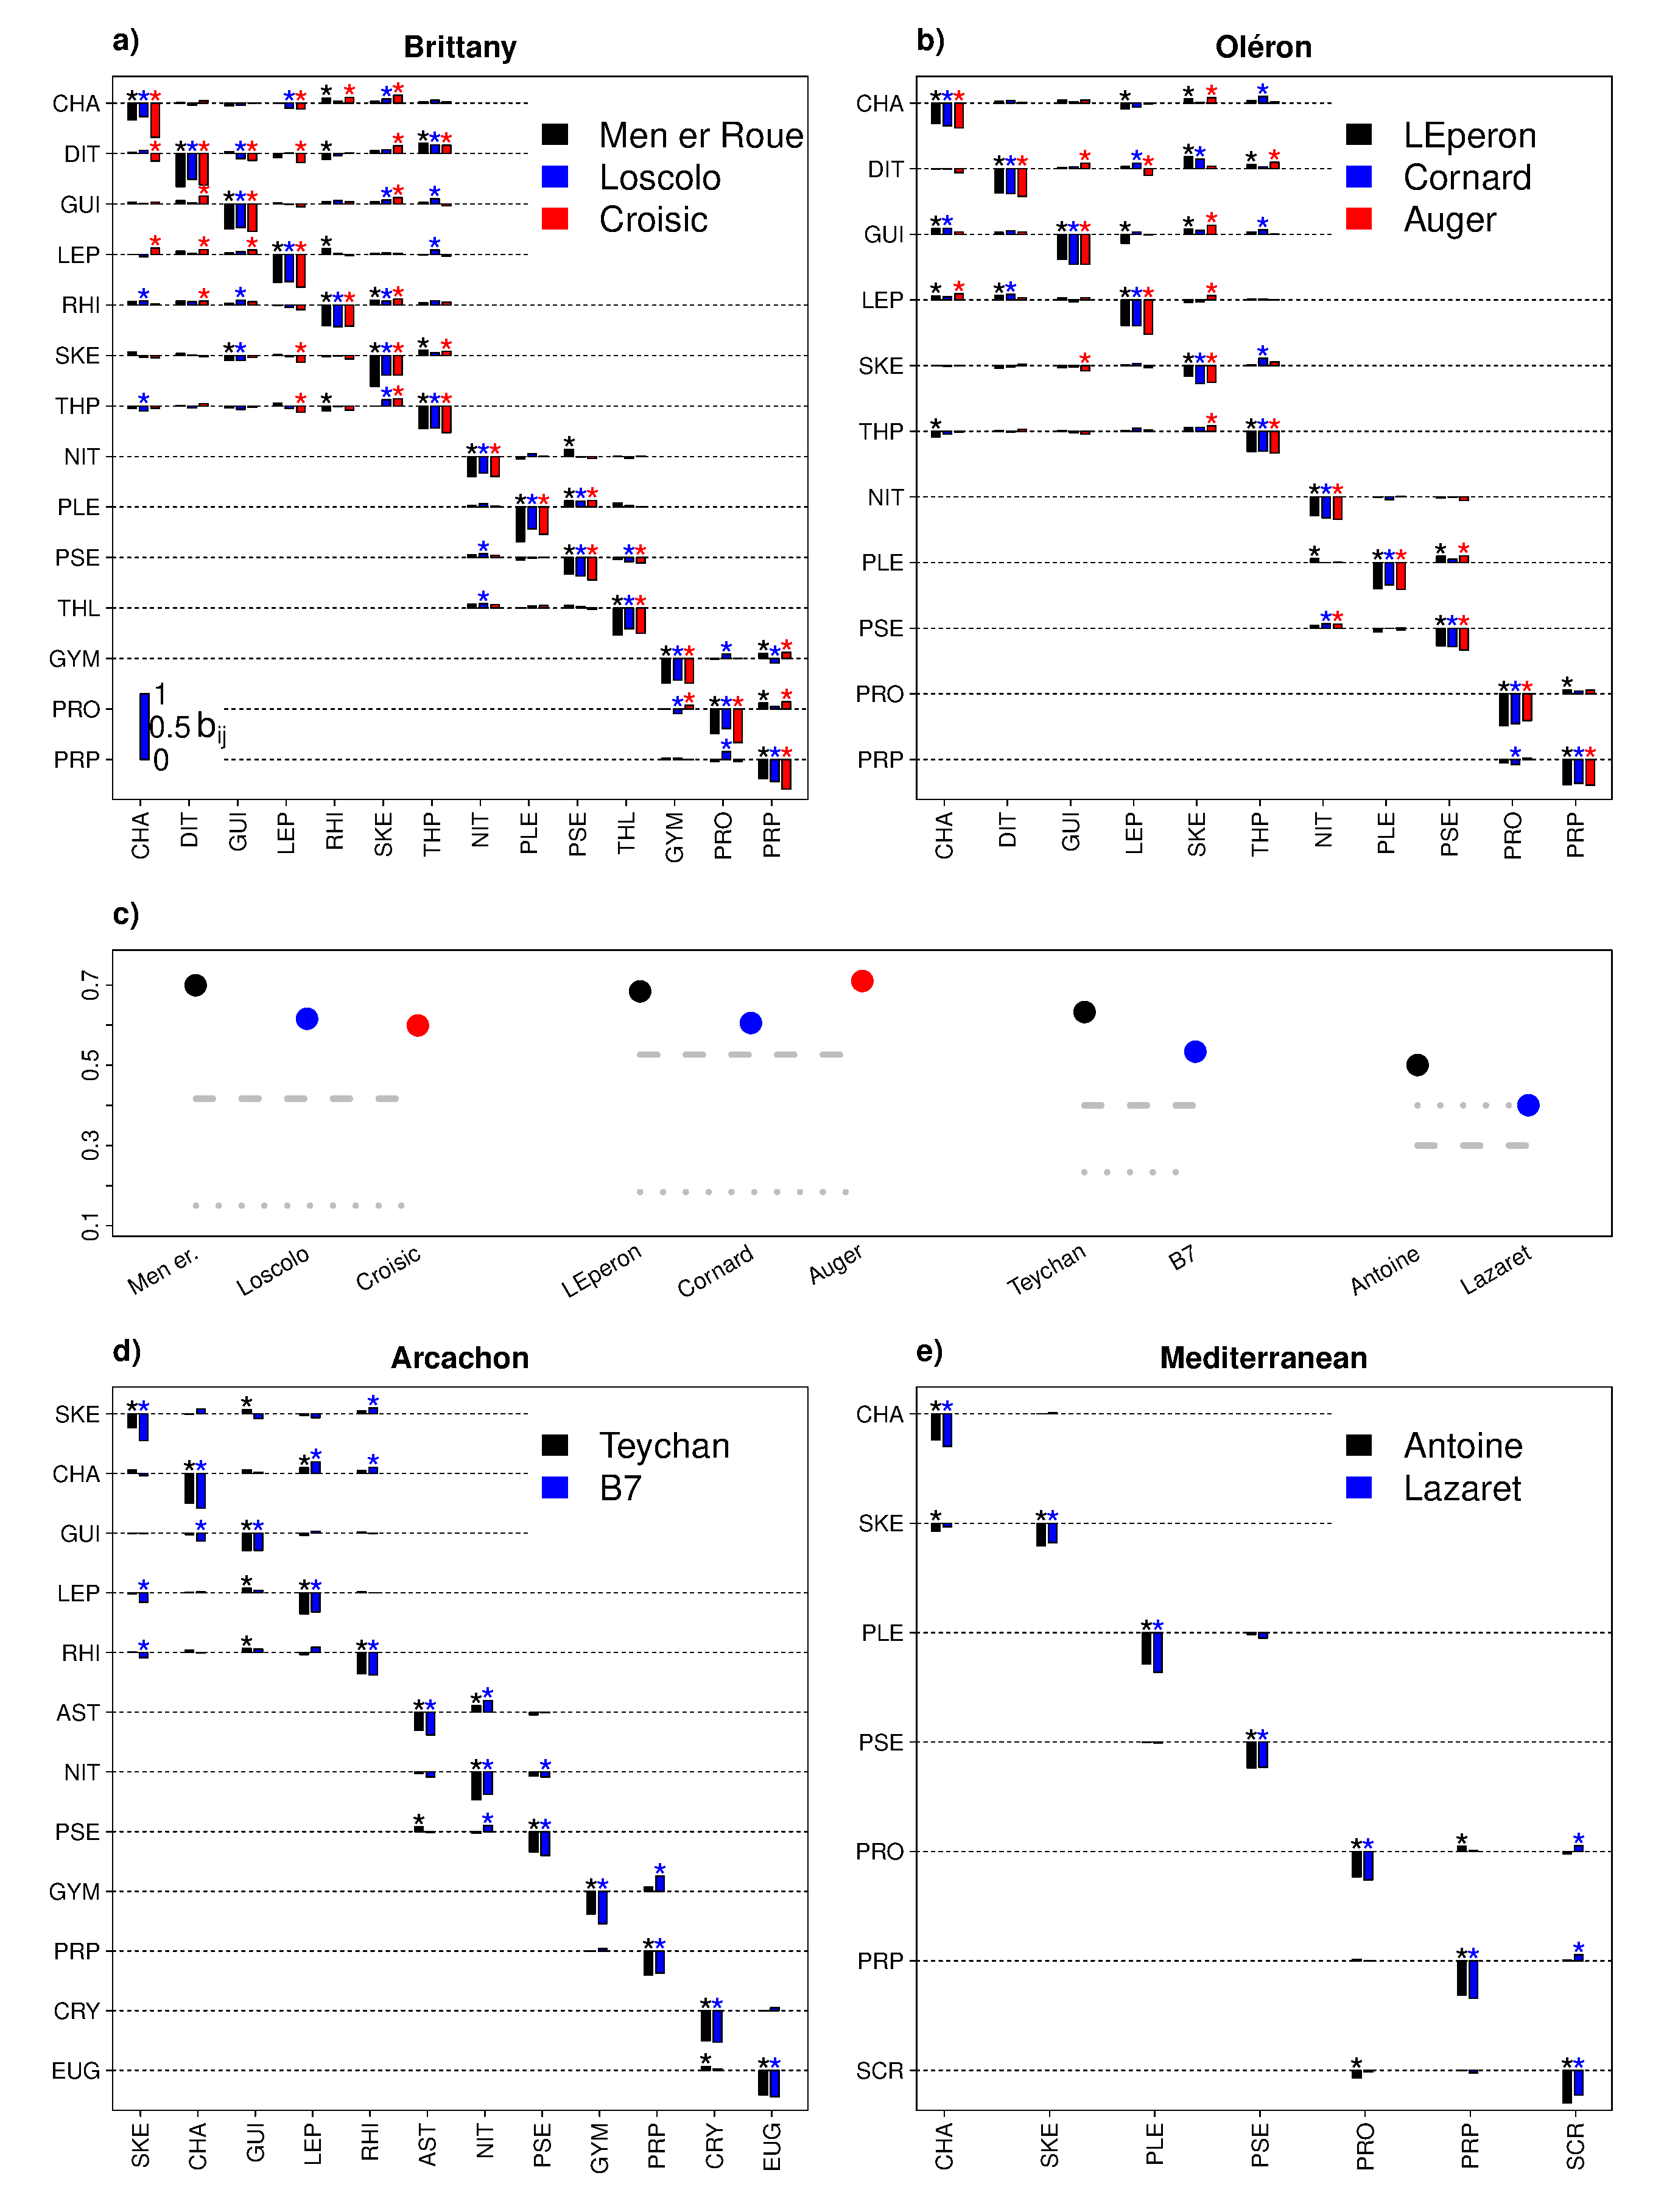
\includegraphics[width=11.4cm]{biotic_interaction_matrices_MainFig_allin1_v4}
% \caption{Interaction matrices estimated in 10 sites along the French
% coastline. Four regions are distinguished: Brittany (a), Oléron (b),
% Arcachon (d) and the Mediterranean Sea (e). Only interactions between
% clades (pennate and centric diatoms, dinoflagellates, other planktonic
% taxa) are allowed, as this is the best fitting interaction scenario
% (Supplementary Fig.~3). Taxon $j$ (in columns) has an effect illustrated
% by the bar height on taxon $i$'s growth rate (in rows). We present
% the interaction matrix minus the identity matrix ($\mathbf{B}-\mathbf{I}$)
% because this compares unambigously intra- and intergenera interactions.
% The scale for the coefficient values is given at the bottom left of
% panel a). 95\% significance of coefficients is marked by asterisks
% ({*}). The community composition is given in Supplementary Table~2.
% The fraction of positive interactions in each matrix is given by points
% in c) while the dashed (resp., dotted) line represents the ratio of
% interactions remaining positive (resp., negative) for all sites of
% a given region.}
% \label{fig:Interaction-matrices}
% \end{SCfigure*}


\matmethods{

\subsection*{Sampling methods}

All phytoplankton counts were collected by Ifremer coastal laboratories
as part of the National Phytoplankton and Phycotoxin Monitoring Network
(REPHY, \citenum{REPHY_db}). Since 1987, this monitoring program
has required the sampling of 26 sites along the French coastline every
2 weeks within 2 hours of high tide to document both biotic (phytoplankton
counts) and abiotic (water temperature, salinity) variables. We focused
on sites which had the longest time series. We also excluded time
series which had missing data for over 6 months or an average delay
between sampling dates above 20 days. This reduced the number of study
sites to 10 sites nested within 4 regions (Brittany, Oléron, Arcachon
and the Mediterranean Sea; SI Appendix, Fig.~S1).

Abiotic variables (temperature, salinity) were measured directly from
the boat during the sampling process while water samples for biotic
analyses were fixed with a Lugol's solution and examined later. Phytoplankton
cells above 20 \textgreek{m}m were identified at the lowest possible
taxonomic level and counted with the Utermöhl method using an optical
microscope \cite{utermohl_zur_1958}. Throughout the years and
sites, more than 600 taxa were identified at different taxonomic levels.
We aggregated them at the genus (or group of genera when not possible)
level based on previous work \cite{hernandez_farinas_assessing_2015,barraquand_coastal_2018},
except for cryptophytes and euglenophytes in Arcachon, which could
not be identified below the family level. Although the taxonomic resolution
used here may seem coarse in comparison to land plants, it is in fact
more refined than 86\% of the MAR(1) studies of phytoplankton listed
in SI Appendix, Table~S3.

For each region, the MAR(1) analysis focused on the most abundant
and most frequently observed genera to avoid most of the gaps in the
time series. When gaps did not exceed a month, missing values were
linearly interpolated; remaining missing values were replaced by a
random number between 0 and half of the lowest observed abundance \cite{hampton_coalescence_2006}. We tested extensively this
and other methods to deal with missing data in a previous publication
on a subset of this dataset \cite{barraquand_coastal_2018}.
All time series were scaled and centered before MAR analyses. All
scripts for MAR and subsequent network analyses are available online
in a GitHub repository\footnote{\texttt{https://github.com/CoraliePicoche/REPHY-littoral} This repository
will be made public upon acceptance and codes can be shared with referees
should they wish to access them.}.

\subsection*{MAR(1) model}

Multivariate autoregressive (MAR) models are used to determine the
interspecific interactions and abiotic effects shaping a community's
dynamics \cite{ives_estimating_2003}. MAR(1) models are based
on a stochastic, discrete-time Gompertz model which relates log-abundance
of $S$ species at time $t+1$ to interactions with the rest of the
community at time $t$, and effects of $V$ abiotic variables at time
$t+1$, following eq. \ref{eq:MAR}.

\begin{equation}
\mathbf{n}_{t+1}=\mathbf{B}\mathbf{n}_{t}+\textbf{C}\textbf{u}_{t+1}+\mathbf{e}_{t},\mathbf{e}_{t}\thicksim\mathcal{{N_{S}}}(0,\mathbf{Q})\label{eq:MAR}
\end{equation}

where $\mathbf{n}_{\ensuremath{t}}$ is the 1$\times$S log abundance
vector of abundance of phytoplankton groups, $\mathbf{B}$ is the
S$\times$S community (interaction) matrix, $\mathbf{C}$ is the S$\times$V
environment matrix describing the effects of V variables (stacked
in vector $\mathbf{u}_{t+1}$) on species growth rates, and $\mathbf{e}_{t}$
is a 1$\times$S noise vector which covers both process and observation
error, following a multivariate normal distribution with a variance-covariance
matrix $\mathbf{Q}$. $\mathbf{Q}$ is diagonal and we have previously
showed that this parsimonious choice did not affect qualitatively
the results \cite{barraquand_coastal_2018}.

We used the MARSS package \cite{holmes_analysis_2014} v3.9, in
R v3.3.2 \cite{venables_r_2013}, to estimate parameters with
a maximum likelihood procedure.

We have previously published a detailed analysis of one of the dataset
(Arcachon) for which more covariables were available \cite{barraquand_coastal_2018},
including nutrients and hydrodynamics variables. We found that hydrodynamics
variables were more influential than nutrients; nutrient dynamics
contributed little to phytoplankton dynamics on the two-week timescale.
Because temperature and salinity sum up seasonal changes in light
as well as hydrology (salinity is inversely related to freshwater
inflow), these represent the two key drivers needed to account for
abiotic influences \cite{scheef_inferring_2013}. The analysis
of real data in Barraquand et al. \cite{barraquand_coastal_2018}
was complemented by that of phytoplankton-like simulated data, which
confirmed the ability of MAR(1) models to infer biotic interactions
and abiotic forcings (e.g., no need for extra non-linearities to model
the storage effect, which was found to be nearly non-existent, as
in previous analyses of plant data for which strong-self regulation
was observed, \citenum{adler_coexistence_2010,ellner_how_2016}).
Furthermore, using two abiotic variables (temperature and salinity)
in this study rather than the full set used in Barraquand et al. \cite{barraquand_coastal_2018}
led to almost identical estimates to the ones obtained previously \cite{barraquand_coastal_2018}.
We are therefore confident that the MAR(1) models presented here are
robust to small changes in model specification. In general, MAR(1)
models tend to be fairly robust to small deviations of the underlying
(non-linear) data-generating model, provided that one asks mainly
order of magnitude of coefficients values (rather than precise point
estimates) and sign of interaction coefficients \cite{certain_how_2018},
which is how these models are used here. For ease of interpretation
of those coefficients, we also prove the correspondance between the
magnitude of intra/inter interaction strength in a MAR(1) model and
a multispecies Beverton-Holt model, i.e., a discrete-time Lotka-Volterra
model, in the SI Appendix.

In this study, the number of phytoplankton groups, S, varies between
regions but we keep the same 2 covariates, i.e. water temperature
and salinity, that were measured at all study sites. Therefore, the
dimension of the dynamical system only depends on the (square of the)
number of phytoplankton groups we study, which ranges between 7 (Mediterranean
Sea) and 14 (Brittany). The smallest system still requires 70 parameters
to be estimated if we consider all possible interactions between species.
To reduce this dimensionality and remove unnecessary parameters, we
compared different `interaction scenarios' based on BIC (SI Appendix
Fig.~S3), which proved to be satisfactory in our previous analyses
of both real data and similar simulated datasets \cite{barraquand_coastal_2018}.
The null interaction scenario assumed no interaction between groups
of species (diagonal interaction matrix) and was compared to four
other interaction scenarios. The first interaction scenario assumed
that interactions could only occur between phylogenetically close
organisms, i.e., within a class (groups were then diatoms, dinoflagellates,
and other phytoplanktonic organisms) while the second interaction
scenario further differentiated pennate and centric diatoms. The third
interaction scenario considered the reverse hypothesis, that only
unrelated organisms could interact (i.e., a diatom could only interact
with a dinoflagellate or a cryptophyte, but not with another diatom),
and the last interaction scenario did not constrain the interactions
at all (full interaction matrix). The second interaction scenario,
hereafter called the pennate-centric scenario, had the lowest BIC
for all sites and was therefore the most parsimonious, and was chosen
as the basis for further investigations of network structure.

\subsection*{Analysis of interaction strengths}

The interaction matrix obtained from MAR(1) analyses can be used to
determine the stability of a discrete-time dynamical system \cite{ives_estimating_2003}.
We compared the maximum modulus of the eigenvalues of the pennate/centric
matrices in each site, as a proxy of stability, to network metrics
which could be related to complexity, such as weighted connectance
and linkage density \cite{breier_emergence_2018}. Weighted connectance
is a measure of the proportion of realized links, taking into account
the shape of the flux distribution, while link density measures the
average proportion and strength of interactions for a given species.
These metrics are adapted to weighted interaction matrices but cannot
accomodate for both positive and negative coefficients: we therefore
chose to focus on the absolute values of these coefficients, which
can be linked to their strength, irrespective of interaction sign.

In addition to these network-level metrics, we also computed the average
vulnerability (average effect of other taxa on a focal taxon, SI Appendix,
Eq.~S5) and impact (average effect of a focal taxon on other taxa,
SI Appendix Eq.~S6) on both raw and absolute values of the coefficients,
and compared these to the regulation a focal species exerted on itself.
Raw values indicate the average effect (i.e., is the effect mostly
positive or negative?) that can be expected on a species' growth rate
from other planktonic species while absolute effects characterise
the strength of all types of interactions on a species (i.e., is a
species strongly affected by the others?). We examined whether vulnerability
and impact could be affected by phylogenetic correlations; they were
not as on Fig.~\ref{fig:Vulnerability_impact} points were not clustered
according to genus, family or phylum.

Finally, we compared our results on the ratio between mean self-regulation/intraspecific
interaction strength and mean interspecific interaction strength to
other published studies based on a MAR(1) model. A list of references
is given in SI Appendix, Table~S3. Authors usually reported only
coefficients that were significant at the 95\% significance threshold,
thus ignoring potentially many weak effects. For mean intergroup interactions,
we therefore computed both the mean value of all coefficients outside
of the matrix diagonal, including zeroes (Fig.~\ref{fig:meta_ratio},
which decreases the mean intergroup interaction strength), and the
mean value of statistically significant intergroup coefficients only
(SI Appendix, Fig.~S8, which increases the mean intergroup interaction
strength). We should mention two potential biases associated with
this comparison across the published literature: low-dimensional matrices
tended to be more complete (less sparse) than high-dimensional matrices,
as these small interaction matrices were used to study known interaction
phenomena (observed predation between organisms, for instance). Conversely,
the number of parameters to estimate increases as the square of the
number of interacting groups, leading most authors to reduce this
set before the estimation process for large interaction matrices.
There is therefore a positive correlation between sparsity and dimensionality
(SI Appendix, Fig.~S9). A second caveat is that while we informed
our model selection by phylogeny (see above), several authors have
reduced the number of estimated parameters by an automated procedure,
usually based on the comparison of 100 randomly chosen interaction
matrices by BIC \cite{ives_estimating_2003}. The latter choice
may bias high non-zero interactions in the literature. This is why
we decided to present in the main text intra/inter ratios including
interspecific (or intergroup) coefficients set to zero, which should
be less sensitive to the model selection method and therefore make
comparisons across studies possible.

}

 \showmatmethods{} % Display the Materials and Methods section

\acknow{This study was only made possible by the dedication of all members of the REPHY program \cite{REPHY_db} by Ifremer, providing invaluable data through years of fieldwork. We are grateful to David Murrell for his careful reading and suggestions, and to Peter Adler for helpful
exchanges. This study was supported by the French ANR through LabEx COTE (ANR-10-LABX-45).}
 
\showacknow{} % Display the acknowledgments section

\subsection*{Supporting Information (SI)}
This article contains supporting information.
% \subsection*{Manuscript Length}
% 
% PNAS generally uses a two-column format averaging 67 characters, including spaces, per line. The maximum length of a Direct Submission research article is six pages and a Direct Submission Plus research article is ten pages including all text, spaces, and the number of characters displaced by figures, tables, and equations.  When submitting tables, figures, and/or equations in addition to text, keep the text for your manuscript under 39,000 characters (including spaces) for Direct Submissions and 72,000 characters (including spaces) for Direct Submission Plus.
% 
% \subsection*{References}
% 
% References should be cited in numerical order as they appear in text; this will be done automatically via bibtex, e.g. \cite{belkin2002using} and \cite{berard1994embedding,coifman2005geometric}. All references should be included in the main manuscript file.  
% 
% \subsection*{Data Archival}
% 
% PNAS must be able to archive the data essential to a published article. Where such archiving is not possible, deposition of data in public databases, such as GenBank, ArrayExpress, Protein Data Bank, Unidata, and others outlined in the Information for Authors, is acceptable.
% 
% \subsection*{Language-Editing Services}
% Prior to submission, authors who believe their manuscripts would benefit from professional editing are encouraged to use a language-editing service (see list at www.pnas.org/site/authors/language-editing.xhtml). PNAS does not take responsibility for or endorse these services, and their use has no bearing on acceptance of a manuscript for publication. 
% 
% % \begin{figure}%[tbhp]
% % \centering
% %  \includegraphics[width=.8\linewidth]{frog}
% % \caption{Placeholder image of a frog with a long example caption to show justification setting.}
% % \label{fig:frog}
% % \end{figure}
% % 
% % 
% 
% % 
% % \subsection*{Digital Figures}
% % 
% % Only TIFF, EPS, and high-resolution PDF for Mac or PC are allowed for figures that will appear in the main text, and images must be final size. Authors may submit U3D or PRC files for 3D images; these must be accompanied by 2D representations in TIFF, EPS, or high-resolution PDF format.  Color images must be in RGB (red, green, blue) mode. Include the font files for any text. 
% % 
% % Figures and Tables should be labelled and referenced in the standard way using the \verb|\label{}| and \verb|\ref{}| commands.
% % 
% % Figure \ref{fig:frog} shows an example of how to insert a column-wide figure. To insert a figure wider than one column, please use the \verb|\begin{figure*}...\end{figure*}| environment. Figures wider than one column should be sized to 11.4 cm or 17.8 cm wide. Use \verb|\begin{SCfigure*}...\end{SCfigure*}| for a wide figure with side captions.
% 
% \subsection*{Tables}
% In addition to including your tables within this manuscript file, PNAS requires that each table be uploaded to the submission separately as a “Table” file.  Please ensure that each table .tex file contains a preamble, the \verb|\begin{document}| command, and the \verb|\end{document}| command. This is necessary so that the submission system can convert each file to PDF.
% 
% \subsection*{Single column equations}
% 
% Authors may use 1- or 2-column equations in their article, according to their preference.
% 
% To allow an equation to span both columns, use the \verb|\begin{figure*}...\end{figure*}| environment mentioned above for figures.
% 
% Note that the use of the \verb|widetext| environment for equations is not recommended, and should not be used. 
% 
% \begin{figure*}[bt!]
% \begin{align*}
% (x+y)^3&=(x+y)(x+y)^2\\
%        &=(x+y)(x^2+2xy+y^2) \numberthis \label{eqn:example} \\
%        &=x^3+3x^2y+3xy^3+x^3. 
% \end{align*}
% \end{figure*}
% 
% 
% \begin{table}%[tbhp]
% \centering
% \caption{Comparison of the fitted potential energy surfaces and ab initio benchmark electronic energy calculations}
% \begin{tabular}{lrrr}
% Species & CBS & CV & G3 \\
% \midrule
% 1. Acetaldehyde & 0.0 & 0.0 & 0.0 \\
% 2. Vinyl alcohol & 9.1 & 9.6 & 13.5 \\
% 3. Hydroxyethylidene & 50.8 & 51.2 & 54.0\\
% \bottomrule
% \end{tabular}
% 
% \addtabletext{nomenclature for the TSs refers to the numbered species in the table.}
% \end{table}
% 
% \subsection*{Supporting Information (SI)}
% 
% Authors should submit SI as a single separate PDF file, combining all text, figures, tables, movie legends, and SI references.  PNAS will publish SI uncomposed, as the authors have provided it.  Additional details can be found here: \href{http://www.pnas.org/page/authors/journal-policies}{policy on SI}.  For SI formatting instructions click \href{https://www.pnascentral.org/cgi-bin/main.plex?form_type=display_auth_si_instructions}{here}.  The PNAS Overleaf SI template can be found \href{https://www.overleaf.com/latex/templates/pnas-template-for-supplementary-information/wqfsfqwyjtsd}{here}.  Refer to the SI Appendix in the manuscript at an appropriate point in the text. Number supporting figures and tables starting with S1, S2, etc.
% 
% Authors who place detailed materials and methods in an SI Appendix must provide sufficient detail in the main text methods to enable a reader to follow the logic of the procedures and results and also must reference the SI methods. If a paper is fundamentally a study of a new method or technique, then the methods must be described completely in the main text.
% 
% \subsubsection*{SI Datasets} 
% 
% Supply Excel (.xls), RTF, or PDF files. This file type will be published in raw format and will not be edited or composed.
% 
% 
% \subsubsection*{SI Movies}
% 
% Supply Audio Video Interleave (avi), Quicktime (mov), Windows Media (wmv), animated GIF (gif), or MPEG files and submit a brief legend for each movie in a Word or RTF file. All movies should be submitted at the desired reproduction size and length. Movies should be no more than 10 MB in size.
% 
% 
% \subsubsection*{3D Figures}
% 
% Supply a composable U3D or PRC file so that it may be edited and composed. Authors may submit a PDF file but please note it will be published in raw format and will not be edited or composed.
% 
% 
% \matmethods{Please describe your materials and methods here. This can be more than one paragraph, and may contain subsections and equations as required. Authors should include a statement in the methods section describing how readers will be able to access the data in the paper. 
% 
% \subsection*{Subsection for Method}
% Example text for subsection.
% }
% 
% \showmatmethods{} % Display the Materials and Methods section
% 
% \acknow{Please include your acknowledgments here, set in a single paragraph. Please do not include any acknowledgments in the Supporting Information, or anywhere else in the manuscript.}
% 
% \showacknow{} % Display the acknowledgments section

% Bibliography
\bibliography{phytoInteractions_ref}
%\bibliography{bib_fig_review}
\end{document}